\section{Introduction}
Video generation models are rapidly evolving from passive content generators into interactive world models~\cite{videoworldsimulators2024, bao2024vidu,wan2025wan,kong2024hunyuanvideo,yang2024cogvideox,lin2024open,zheng2024open,sun2025worldplay,genie3,huang2025live,ki2026avatar,sun2025streamavatar,feng2025vidarc,ye2026worldactionmodelszeroshot}, where low latency, streaming rollout, and user-controllable interaction are essential. Autoregressive (AR) diffusion models~\cite{jin2024pyramidal,teng2025magi,chen2025skyreels} are a natural fit for this goal, as they perform causal rollout across frames or chunks while retaining diffusion-based generation within each segment. Recent AR diffusion distillation methods~\cite{yin2025slow,huang2025self,zhu2026causal,huang2025live,sun2025worldplay} have achieved promising results by distilling bidirectional video diffusion models, such as Wan~\cite{wan2025wan} and Hunyuan~\cite{kong2024hunyuanvideo}, into few-step AR students. However, these methods typically rely on chunk-wise autoregression with 4-step sampling, which still falls short of real-time interaction due to coarse response granularity and non-negligible sampling latency.  We therefore push AR diffusion distillation to a more aggressive and largely underexplored regime: \emph{frame-wise autoregression with only 1--2 sampling steps}.

We identify the initialization of a few-step AR student before asymmetric DMD as the key bottleneck in this aggressive regime, where existing strategies fail in complementary ways. ODE initialization with a bidirectional teacher, as used in CausVid~\cite{yin2025slow} and Self Forcing~\cite{huang2025self}, is architecturally misaligned with causal rollout: the teacher trajectory depends on future frames that are unavailable to an AR student, thereby providing an incorrect regression target. Directly using a multi-step AR diffusion model for initialization, as in LiveAvatar~\cite{huang2025live} and WorldPlay~\cite{sun2025worldplay}, avoids this mismatch but lacks few-step generation capability; under frame-wise 1--2 step generation, its per-frame approximation error is severely amplified during self-rollout. Causal ODE initialization, as in Causal Forcing~\cite{zhu2026causal}, corrects the learning target by distilling from an AR teacher, but requires generating full multi-step PF-ODE trajectories for every training sample, making it costly to scale. Therefore, a satisfactory initialization for this regime must be simultaneously \emph{AR}, \emph{few-step}, and \emph{scalable}.

To this end, we introduce \textbf{Causal Forcing++}, a principled and scalable pipeline that uses \emph{causal consistency distillation} (causal CD) for few-step AR student initialization. Our key observation is that causal ODE distillation and causal CD aim to learn the same object: the AR-conditional flow map (or namely the consistency function~\cite{song2023consistency,wang2024phased,lu2024simplifying,zheng2025large}) of the teacher. They differ, however, in how the supervision is obtained. Causal ODE distillation requires the AR teacher to generate an entire multi-step PF-ODE trajectory for each training sample, which must be precomputed and stored offline. In contrast, causal CD obtains supervision from a single online teacher ODE step between adjacent timesteps on real videos. Therefore, causal CD serves as a principled substitute for causal ODE initialization, while avoiding the expensive trajectory-generation bottleneck. Beyond efficiency, this local supervision also improves quality: adjacent-timestep consistency yields a smaller per-step optimization gap than causal ODE distillation, which regresses noisy intermediate states directly to clean endpoints~\cite{liu2023instaflow}. As a result, causal CD is easier to optimize and empirically produces a stronger few-step AR student.

Experiments on Wan2.1-1.3B~\cite{wan2025wan} validate the effectiveness of Causal Forcing++ in this aggressive low-latency regime. Under frame-wise 2-step generation, Causal Forcing++ achieves the best overall performance among existing AR diffusion distillation methods, improving VBench Total, VBench Quality, and VisionReward over prior methods while reducing first-frame latency by 50\%. Ablation studies further show that causal CD consistently matches or outperforms causal ODE initialization across 1-step, 2-step, and 4-step settings, while reducing the Stage 2 cost by about $4\times$ and requiring no auxiliary trajectory storage. We also examine causal score-distillation initialization and find that, although it can produce sharper early frames, its mode-seeking behavior makes it more sensitive to accumulated history errors during AR rollout, leading to stronger exposure bias. Finally, we demonstrate that Causal Forcing++ naturally extends to action-conditioned world model generation by distilling a camera-pose-conditioned generator into an interactive AR world models. 





\begin{figure}[htbp]
    \centering
    \vspace{-.25cm}
    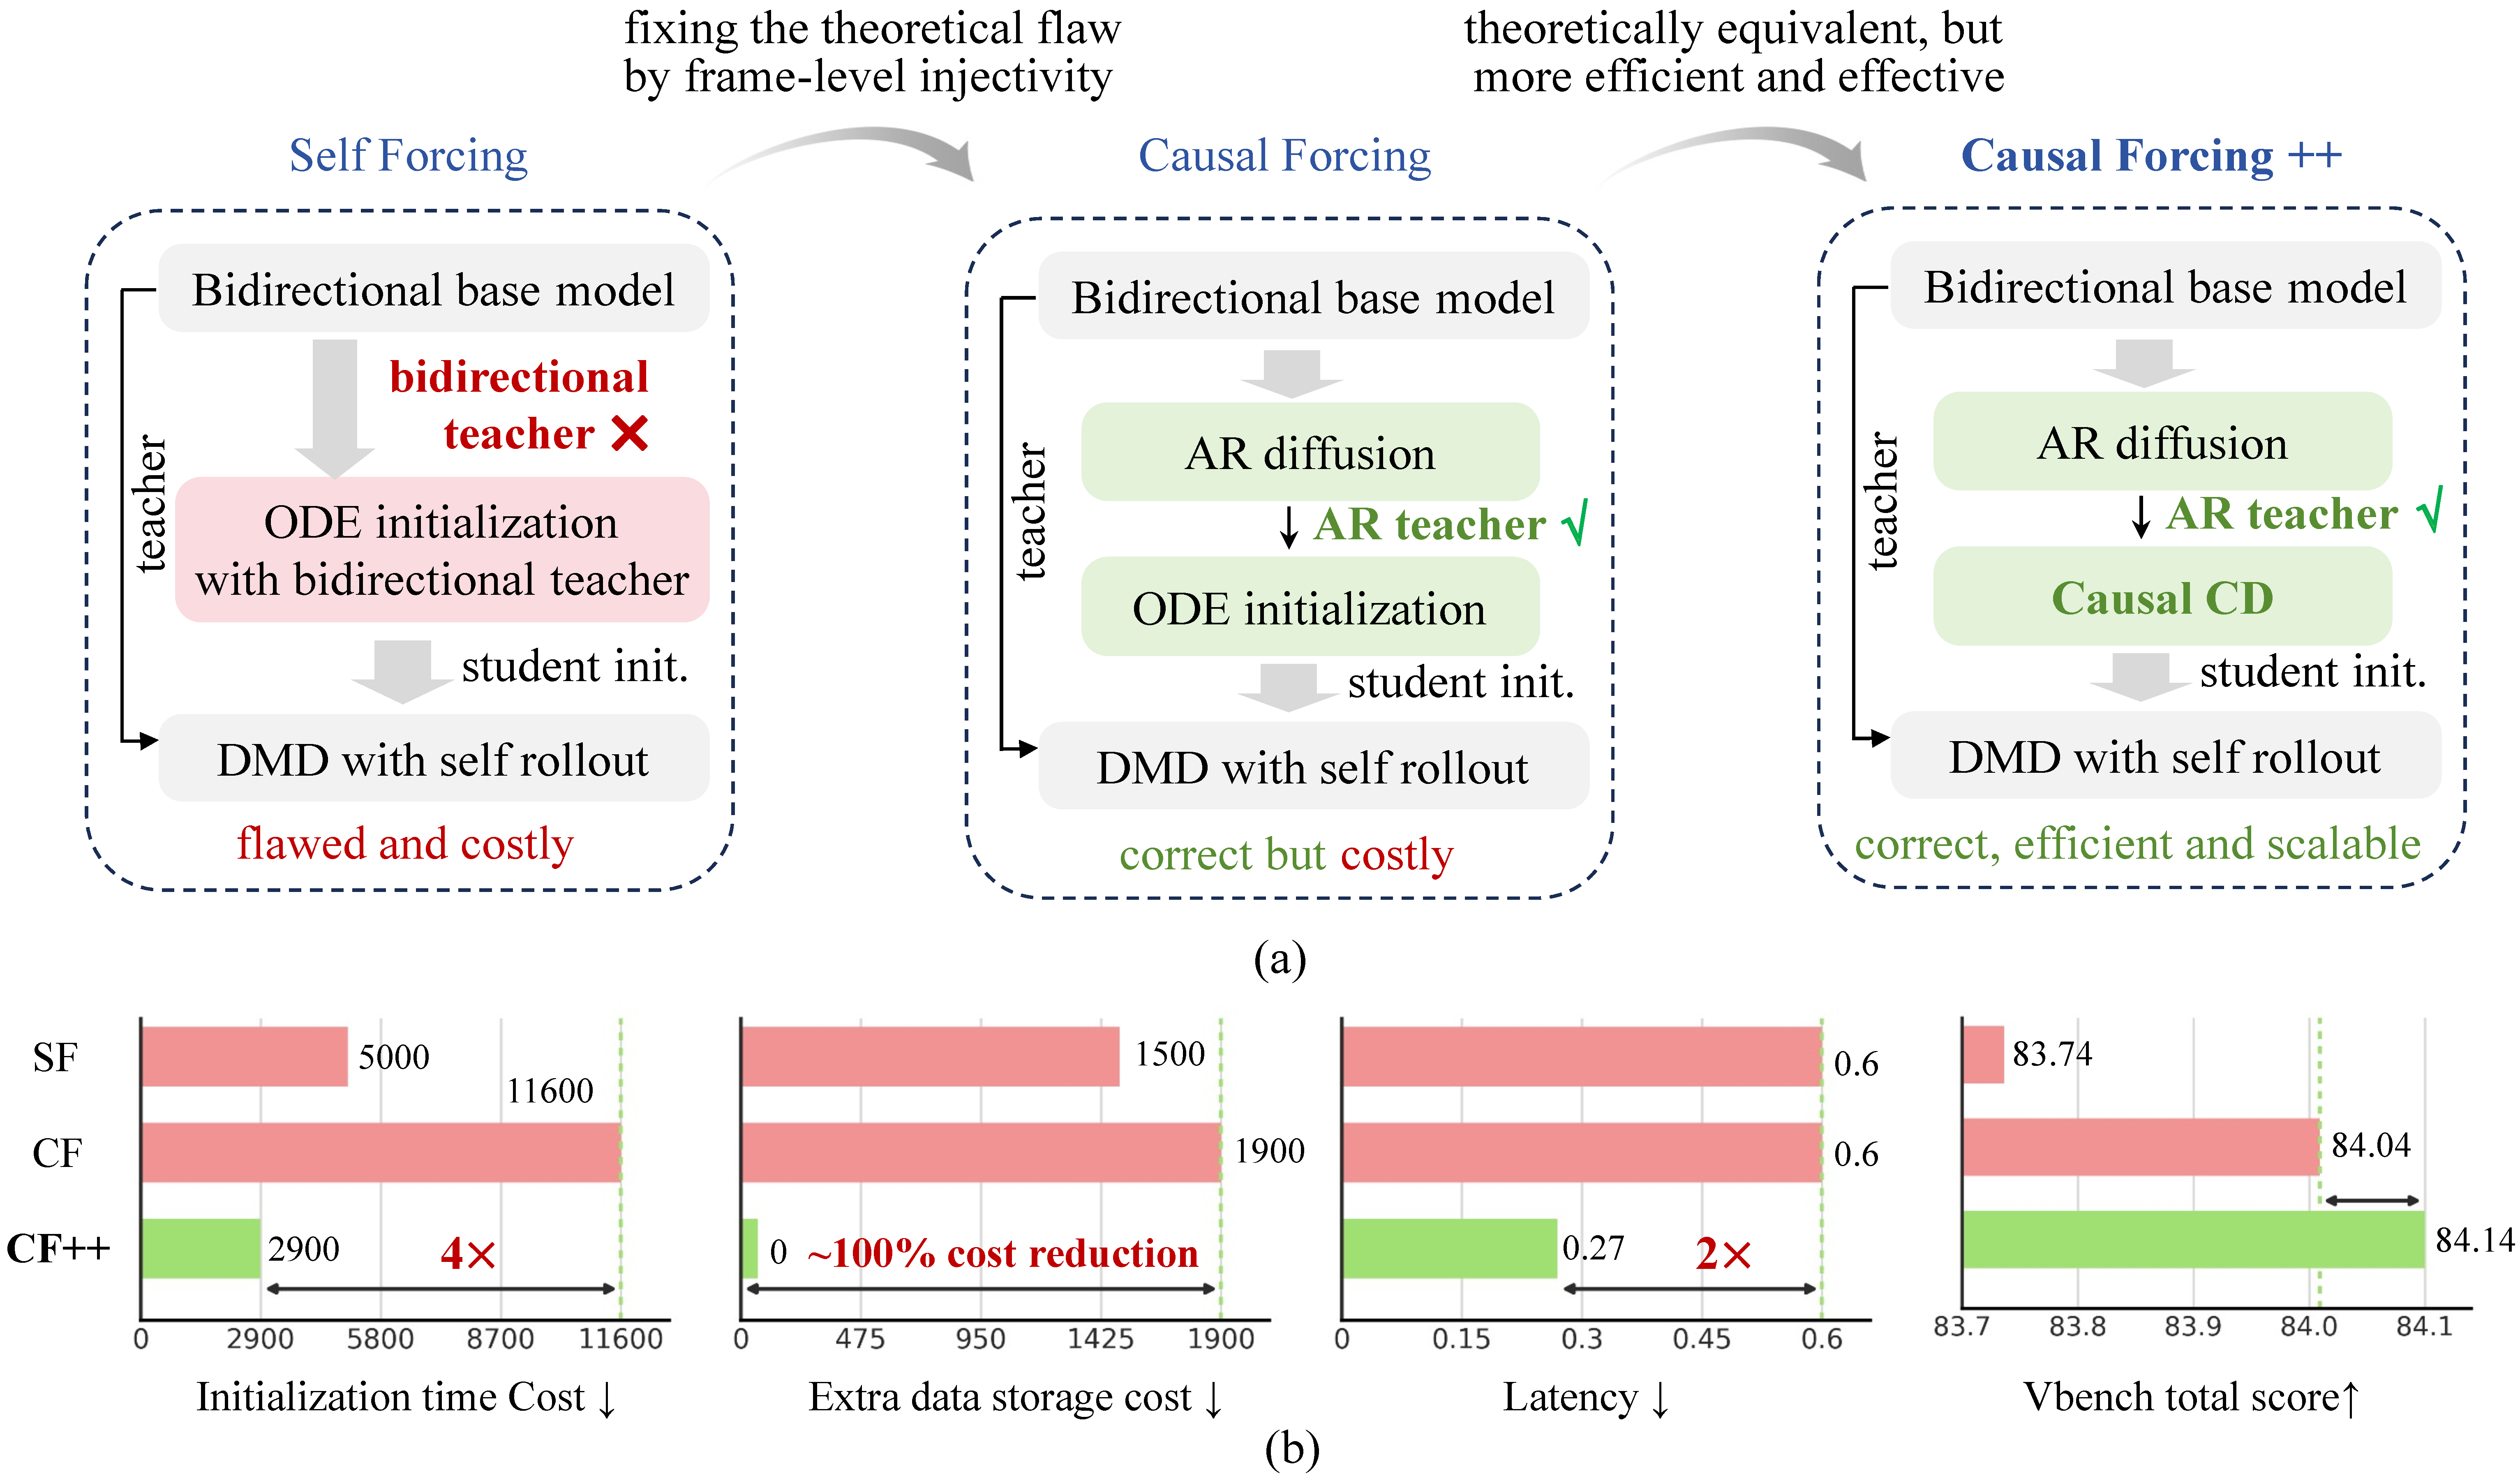
\includegraphics[width=\textwidth]{Figures/overall.pdf}
    \vspace{-.2cm}
    \caption{\textbf{Overall framework of our Causal Forcing++ and the comparison with existing methods.} (a) Causal Forcing (CF) fixes Self Forcing (SF)'s frame-level injectivity flaw but remains costly; our Causal Forcing++ (CF++) is theoretically sound, efficient, and scalable. (b) Our CF++ reduces training cost by 4$\times$, requires no extra data curation, and achieves 50\% lower latency and higher VBench scores than SF and CF.}
    \label{fig:overall}
    \vspace{-.5cm}
\end{figure}

